\documentclass[10pt]{article}
\usepackage{amsmath, amssymb, amsfonts} % برای فرمول‌نویسی
\usepackage{breqn} % برای فرمول‌نویسی
\usepackage{amsthm}% برای اضافه کردن محیط proof
\usepackage{subfigure} % اضافه کردن شکل های زیر شکل ها
\usepackage{setspace} % تعیین فاصله بین خطوط
\usepackage{graphicx} % اضافه کردن عکس
\usepackage{multicol} % حروف چینی چند ستونه
\usepackage[margin=1in]{geometry} % تغییر دادن حاشیه دور
\usepackage{fancyvrb}
\usepackage{tcolorbox}

\graphicspath{{./pics/}}

\usepackage{xepersian}

\settextfont{XB Yas} % برای ست کردن فونت متن
\setdigitfont{XB Zar} % برای ست کردن فونت اعداد

\setcounter{secnumdepth}{4} % Set Sections' Depth
\setcounter{tocdepth}{4}% Set Table Of Content's Depth

\title{تمرین کامپیوتری ۲ سیستم‌های مخابراتی}
\author{نام و نام‌ خانوادگی : امیرمهدی جعفری فشارکی
\\ \\
شماره دانشجویی : ۹۸۱۰۹۶۴۵ 	\\ \\
تاریخ : ۷ دی ۱۴۰۰ }
\date{}
\doublespacing

\begin{document}
	\maketitle
	\pagebreak
	\newpage
	\section*{توضیحات اولیه}
	کد‌های مربوط به سوالات در فولدر 
	\lr{Codes}
	قرار دارد و تمامی تصاویر مربوط به سوالات در فولدر 
	\lr{pics}
	قرار دارد.
	همچنین این گزارش با استفاده از
	 \LaTeX
	 تهیه شده است و فایل 
	 \lr{tex}
	 مربوط به آن در فولدر 
	 \lr{Report}
	 قرار دارد.
	\section{\lr{Envelope Detector}}
	کد‌ مربوط به این سوال در 
	\lr{Q1.m}
	قرار داد. همچنین تابع مورد نظر برای بخش دوم در فایل 
	\lr{EnvelopeDetector.m}
	قرار دارد و کد آن مطابق زیر می‌باشد.
	\begin{latin}
	\begin{tcolorbox}
\begin{Verbatim}[tabsize=4]
function [out] = EnvelopeDetector(x, t, r, c)
%This function finds the envelope of a signal for a given R and C
out = zeros(1, length(t));
local_peak = 0;
t_peak = 0;
for i=1:length(t)
	out_exp = local_peak * exp(-(t(i) - t_peak)/(r * c));
	if out_exp < x(i)
		local_peak = x(i);
		t_peak = t(i);
		out(i) = x(i);
	else
		out(i) = out_exp;
	end
end
\end{Verbatim}
	\end{tcolorbox}
	\end{latin}
\noindent
	 در بخش سوم نیز، از مقادیر زیر به عنوان مقادیر پارامترهای 
	\lr{R}
	و
	\lr{C}
	استفاده شده است.
	\[
	R = 1k\Omega \quad C = 42 \mu F
	\]
	\newpage
	\noindent
	در ادامه با استفاده از مقادیر ذکر شده، نمودار‌های خواسته شده هم در یک نمودار و هم به صورت جداگانه رسم شده است. سیگنال‌های مورد نظر در دو نمودار زیر هم به صورت جداگانه و هم روی هم رسم شده اند.
	
\begin{figure}[h]\label{fig:q1}
	\begin{center}
		\subfigure[نمودار سیگنال‌ها به صورت جداگانه]{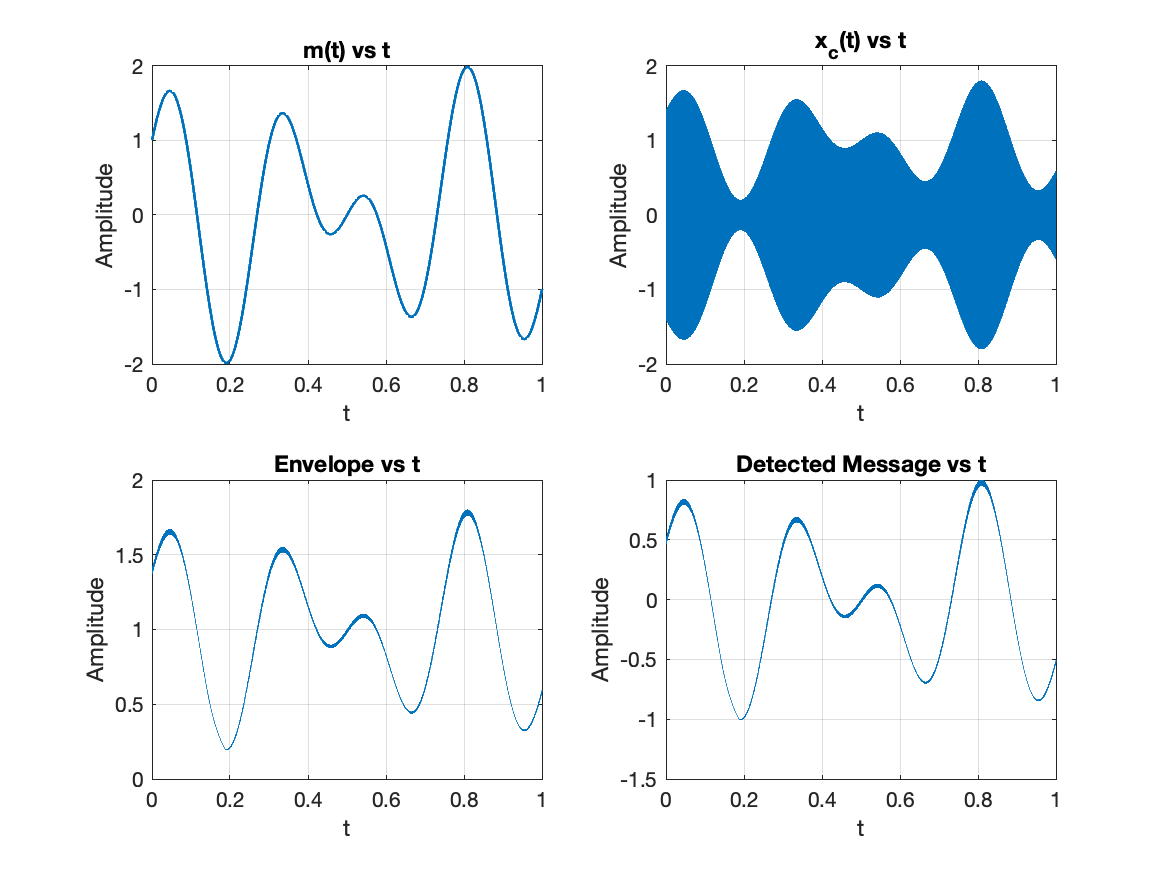
\includegraphics[width=0.45\linewidth]{../pics/q1-1.png}}
		\hspace{0.03\linewidth}
		\subfigure[نمودار سیگنال‌ها روی هم]{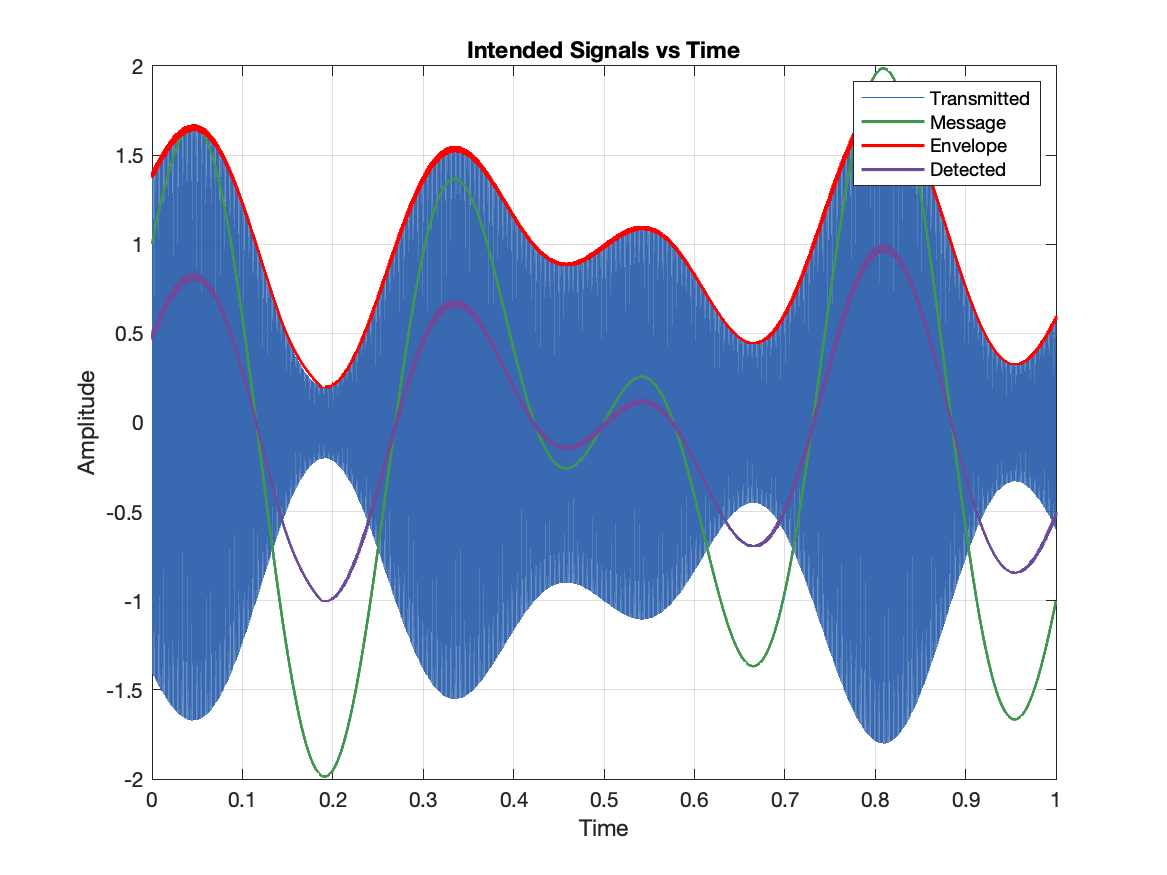
\includegraphics[width=0.45\linewidth]{../pics/q1-2.png}}
	\end{center}
	\caption{نمودار سیگنال‌های خواسته شده}
\end{figure}

\noindent
همچنین لازم به ذکر است که سیگنال استخراج شده با سیگنال پیام فقط در اندازه دامنه خود فرق دارند و دلیل این موضوع این است که سیگنال استخراج شده با سیگنال پیام نرمالیزه شده برابر است (چرا که در ابتدا نرمالیزه این سیگنال را به عنوان پیام مدوله کردیم.). به همین دلیل در نمودار شکل زیر، ماکسیمم اندازه پیام اصلی در پیام استخراج شده تا این موضوع بهتر مشاهده شود.
\begin{figure}[h]
	\centering
	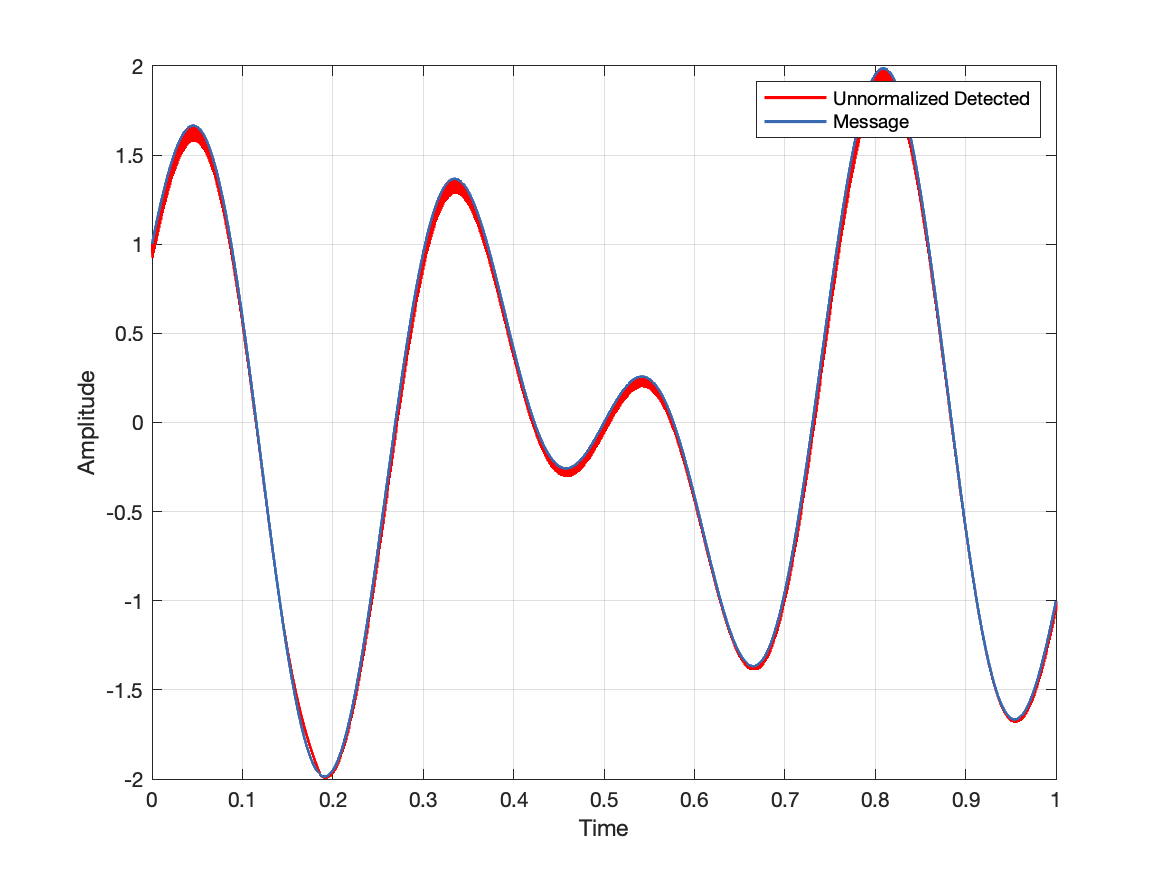
\includegraphics[width=0.7\linewidth]{../pics/q1-3}
	\caption{مقایسه پیام اصلی با پیام استخراج شده ضرب شده در دامنه ماکسیمم پیام اصلی}
	\label{fig:q1-3}
\end{figure}
\newpage

\section{\lr{USSB Modulation}}
کد مربوط به این سوال در فایل 
\lr{Q2.m}
قرار گرفته است. در بخش اول کد، از سیگنال های گفته شده با فرکانس 
$f_s = 10000Hz$
نمونه برداری شده است. سپس در بخش دوم با استفاده از دستور 
\lr{ssbmod}،
سیگنال های بخش قبل با فرکانس‌های مرکزی مختص خود مدوله شده اند. 
\subsection*{سیگنال های پیام، مدوله شده و فرستاده شده بر حسب زمان}
در بخش سوم نمودار پیام‌ها، سه سیگنال مدوله شده و سیگنال ارسالی که حاصلجمع سه سیگنال مدوله شده است، رسم شده است و در شکل زیر قابل مشاهده است.
\begin{figure}[h]
	\centering
	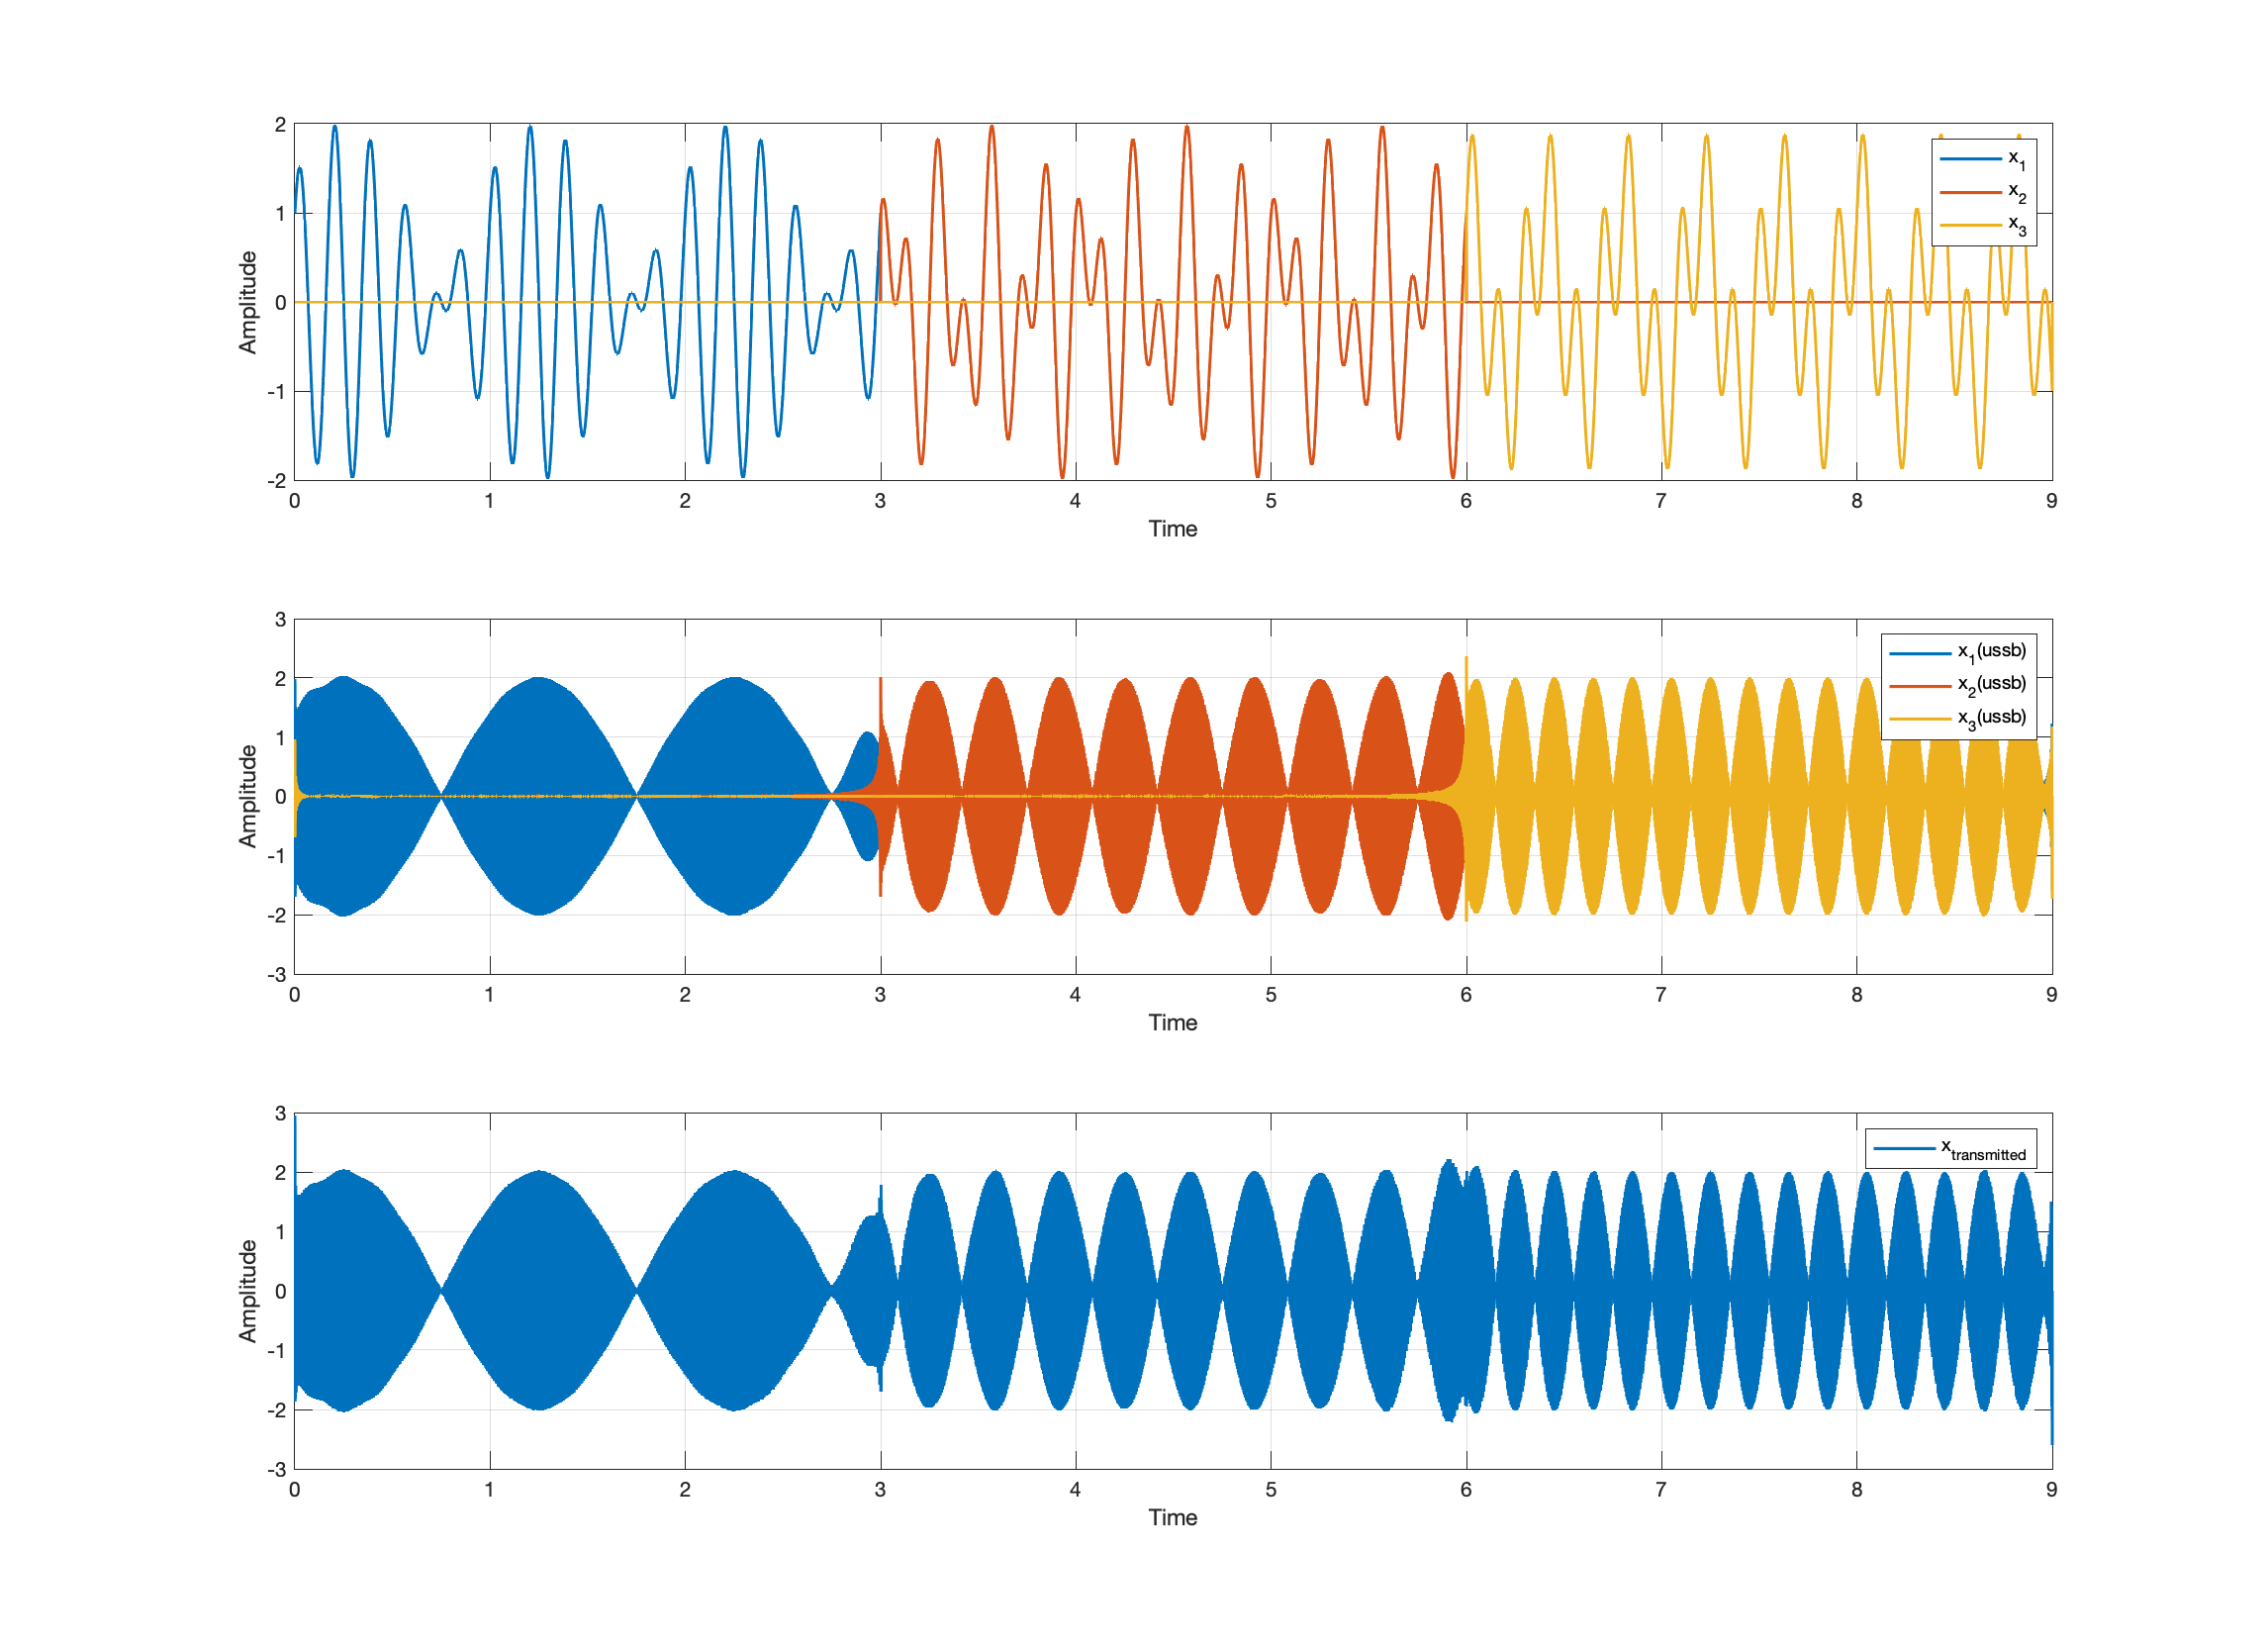
\includegraphics[width=0.95\linewidth]{../pics/q2-1}
	\caption{نمودار سیگنال‌های خواسته شده}
	\label{fig:q2-1}
\end{figure}

\newpage
\subsection*{تبدیل فوریه سیگنال‌های پیام، مدوله شده و فرستاده شده}
\noindent
نمودار تبدیل فوریه سیگنال‌های خواسته شده مطابق شکل زیر می‌باشد. لازم به ذکر است که برای مشاهده بهتر سیگنال های پیام اصلی، اسکیل نمودار آن ها کوچکتر از بقیه نمودار ها می‌باشد.
\begin{figure}[h]
	\centering
	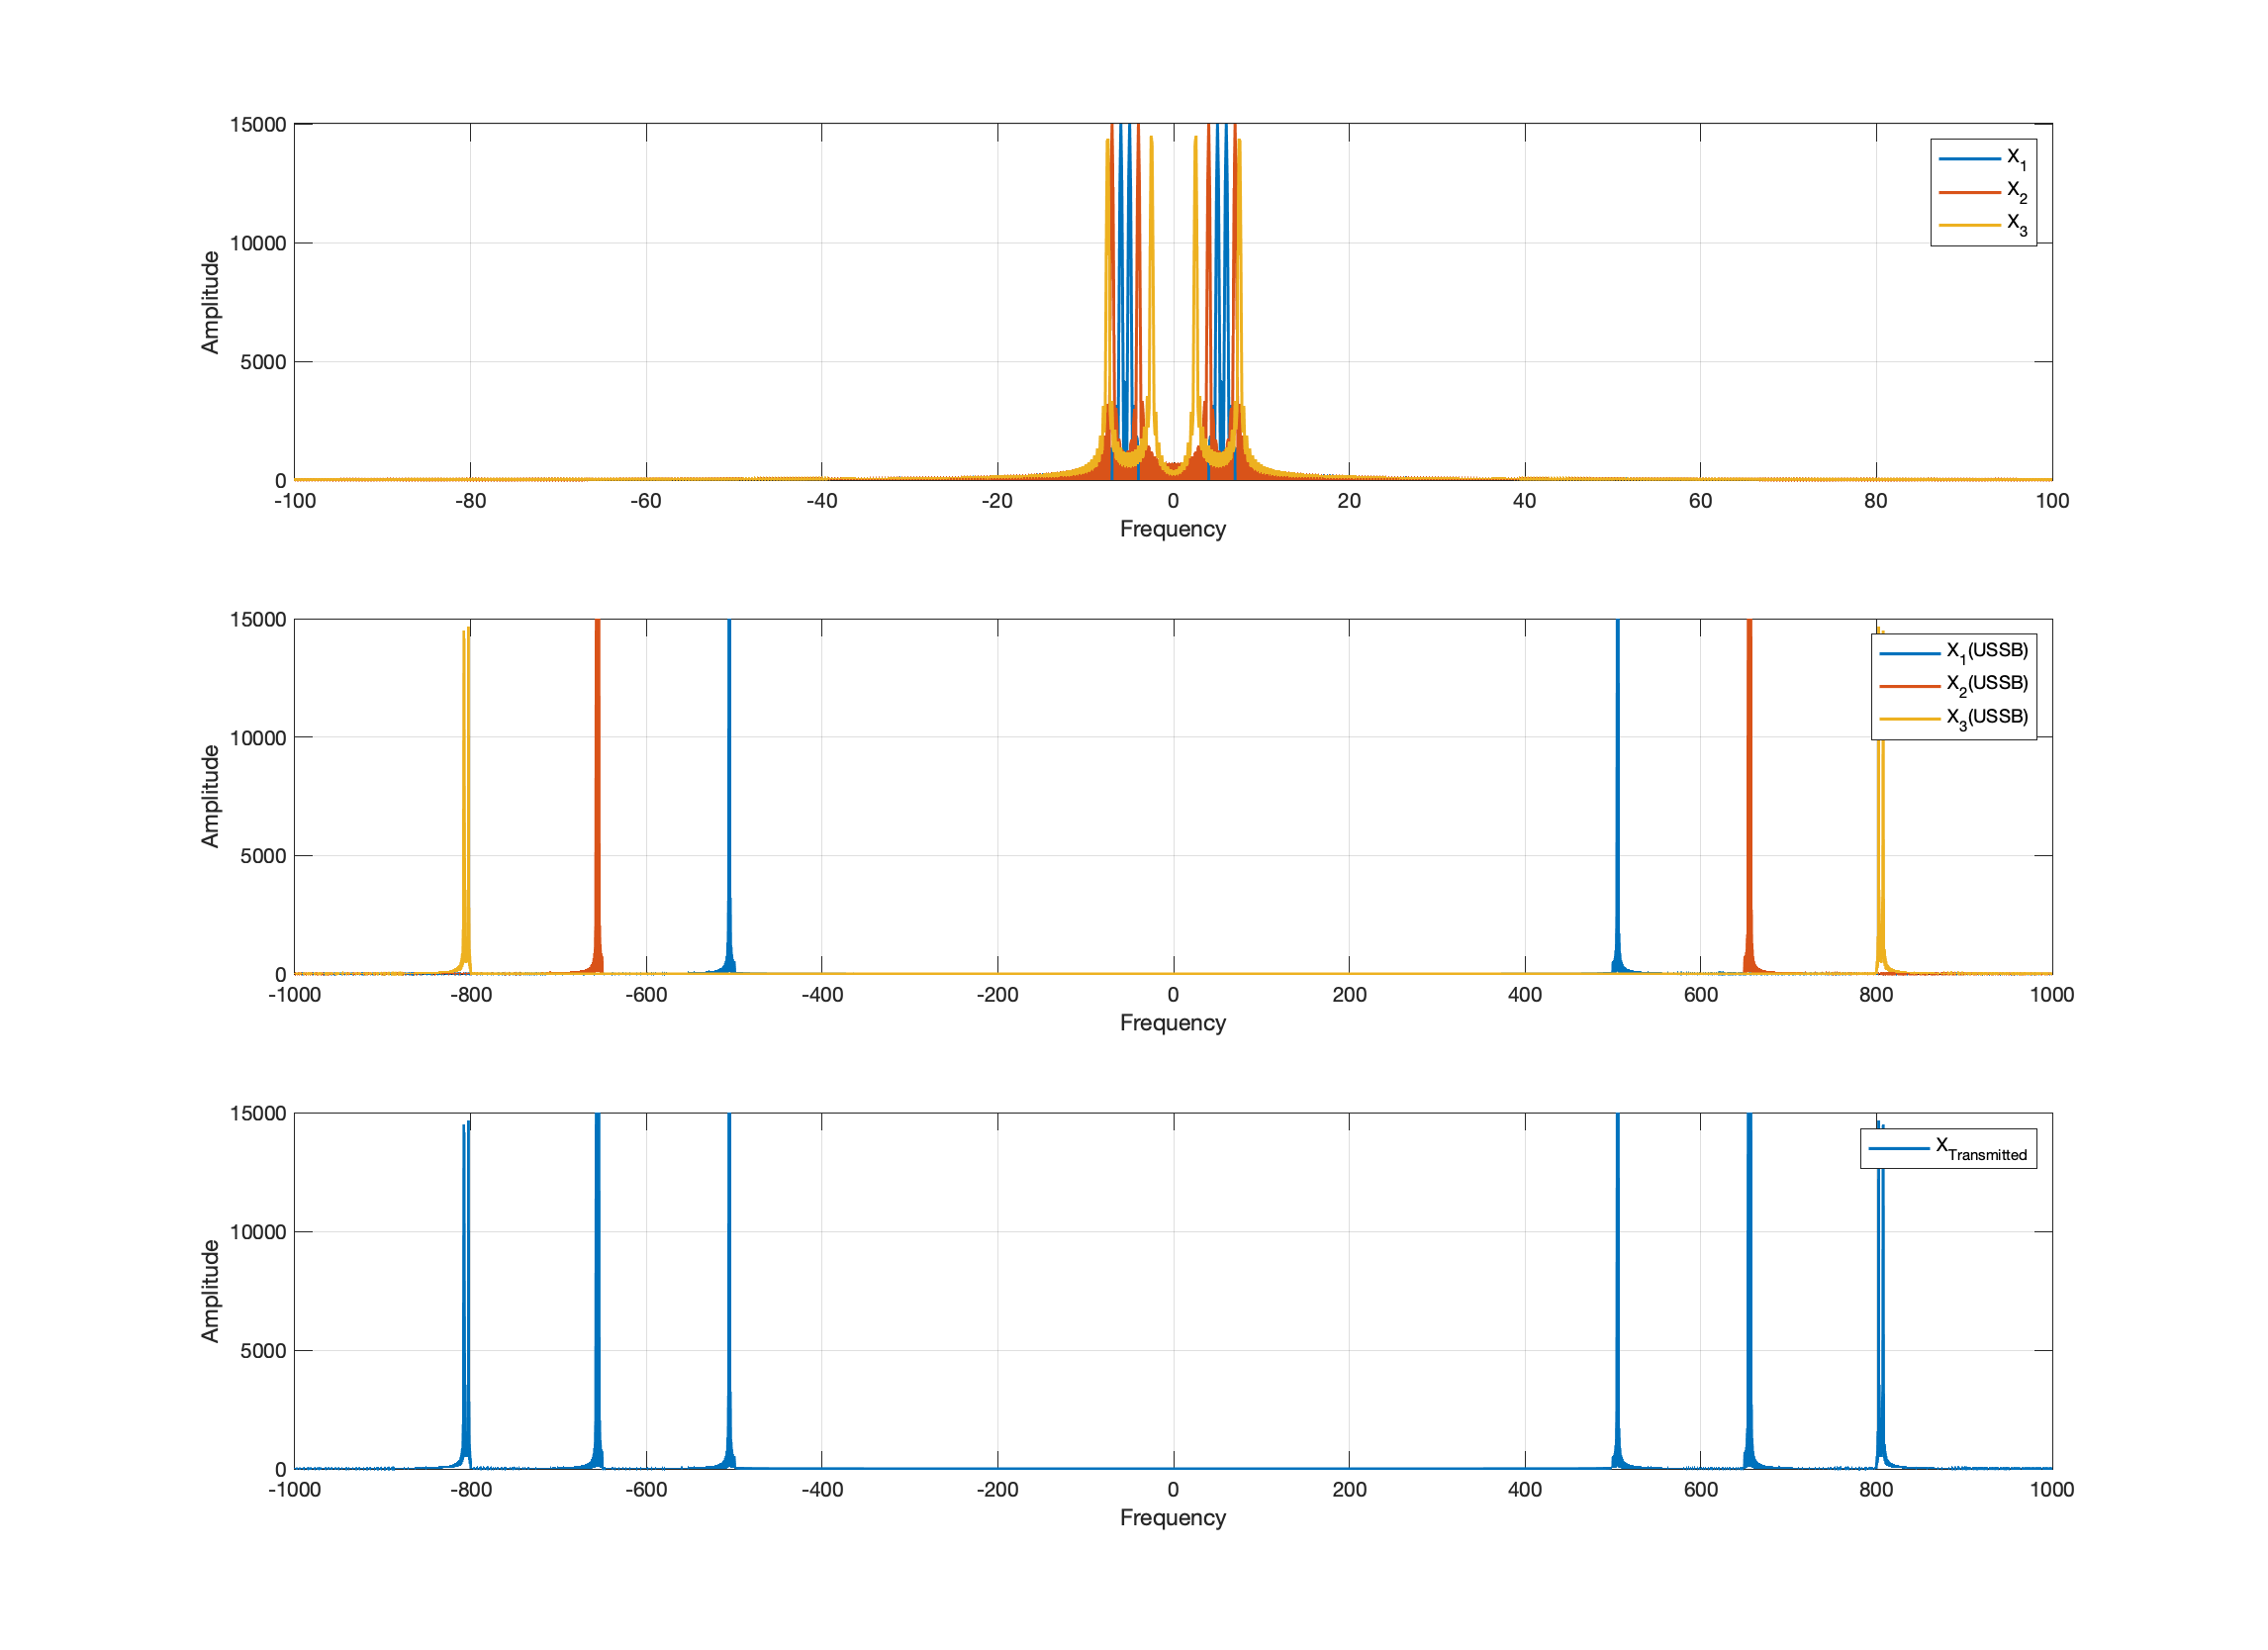
\includegraphics[width=0.95\linewidth]{../pics/q2-2}
	\caption{نمودار تبدیل فوریه سیگنال‌های خواسته شده}
	\label{fig:q2-2}
\end{figure}

\noindent
در بخش پنجم، برای اضافه کردن نویز با 
\lr{SNR = 5dB}
از یک نویز گوسی رندوم استفاده شده است که در انحراف معیار سیگنال فرستاده شده ضرب و بر 
\lr{SNR}
 مورد نظر تقسیم شده است چرا که انحراف معیار در حقیقت برای این سیگنال گسسته برابر با توان سیگنال تقسیم بر طول سیگنال (تعداد نمونه ها) می‌باشد. برای پیاده سازی این نویز ذکر شده از قطعه کد زیر استفاده شده است.
\begin{latin}
\begin{tcolorbox}
\begin{Verbatim}
SNR = 5;
noise = randn(size(t)) * std(x_trans)/db2mag(SNR);
x_channel = x_trans + noise;
\end{Verbatim}
\end{tcolorbox}
\end{latin}
\newpage
\noindent
\subsection*{تبدیل فوریه سیگنال دریافت شده و سیگنال فیلتر شده}
پس از اعمال نویز مورد نظر، با استفاده از یک فیلتر میان‌گذر، نویز‌های خارج از باند فرکانسی سیگنال ارسالی حذف شده و در نهایت نمودار تبدیل فوریه سیگنال دریافت شده و سیگنال فیلتر شده مطابق شکل زیر رسم شده است.
\begin{figure}[h]
	\centering
	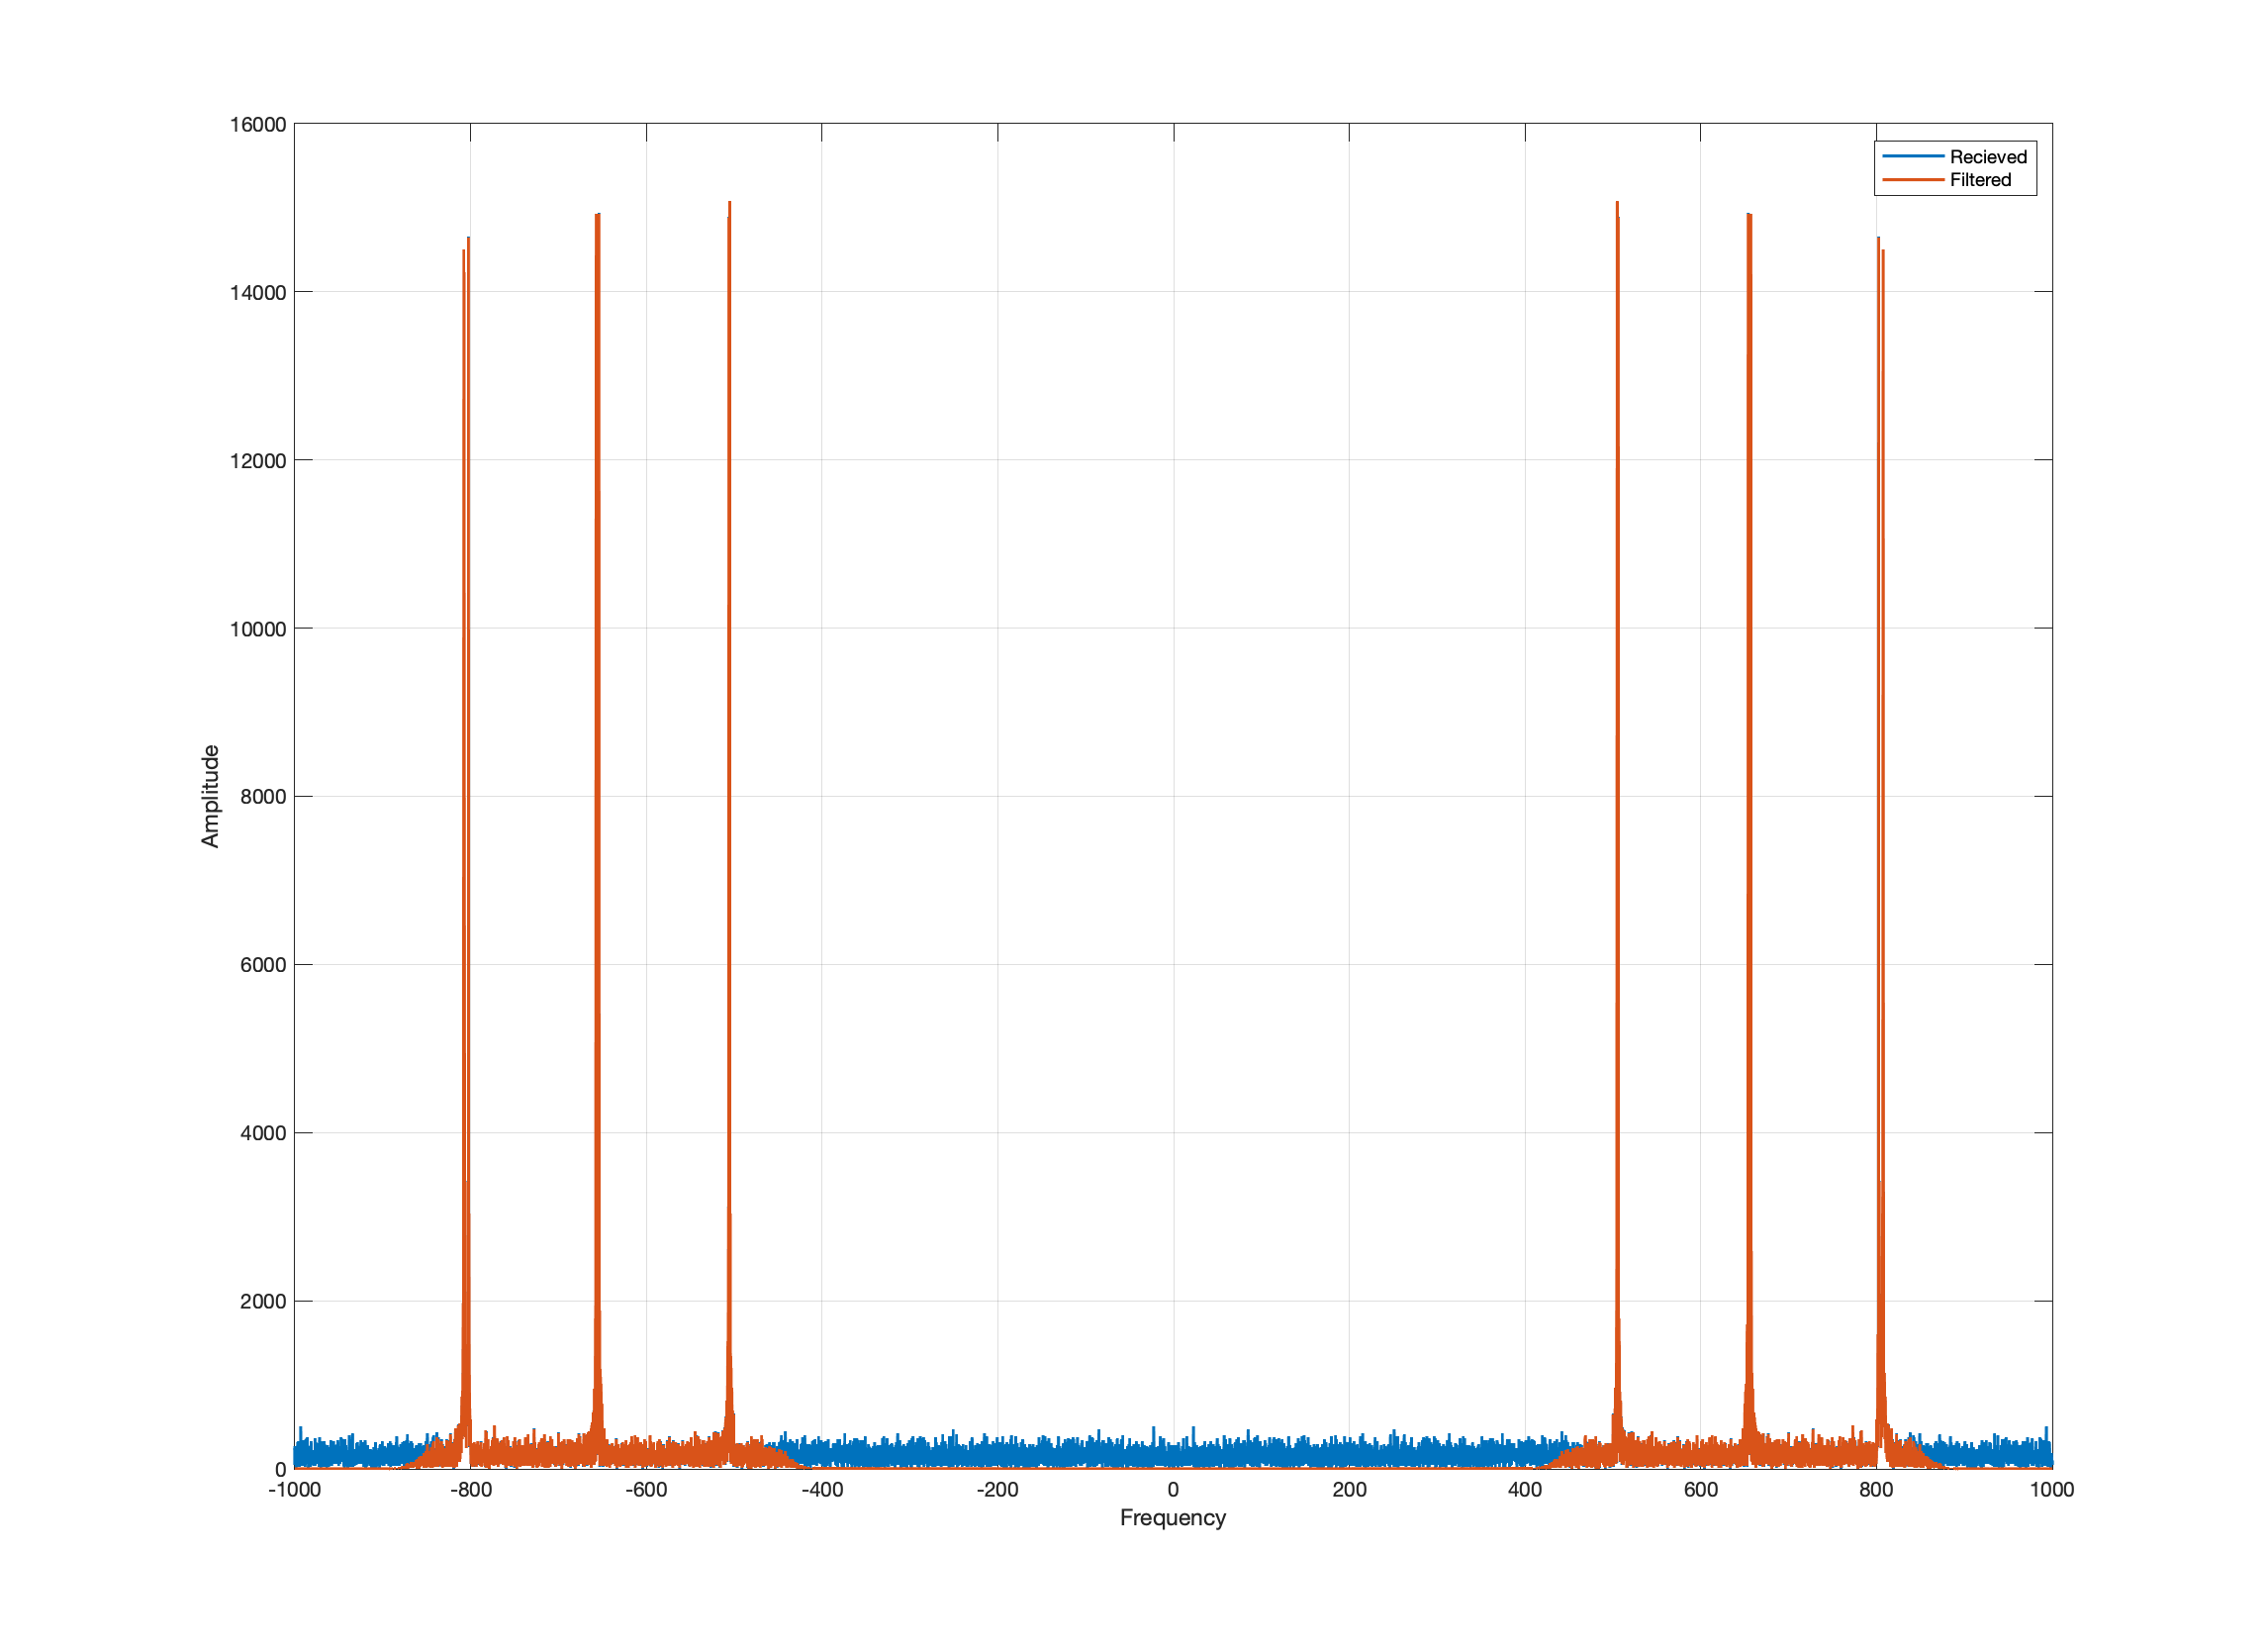
\includegraphics[width=0.95\linewidth]{../pics/q2-3}
	\caption{نمودار اندازه تبدیل فوریه سیگنال نویزی دریافت شده و سیگنال فیلتر شده }
	\label{fig:q2-3}
\end{figure}

\newpage
\subsection*{مقایسه سیگنال‌های پیام فرستاده و دریافت شده}
در ابتدا برای هر کدام از پیام‌ها، با استفاده از یک فیلتر میان‌گذر، بخش مورد نظر از هر سیگنال انتخاب شده و سپس توسط دستور 
\lr{ssbdemod}
دمدوله شده است. در نهایت پیام‌های ارسالی و دریافتی مطابق شکل زیر هم روی هم و هم برای بررسی بیشتر به صورت جدا از هم رسم شده اند.
\begin{figure}[h]\label{fig:q2-5}
	\begin{center}
		\subfigure[نمودار سیگنال‌ها به صورت جداگانه]{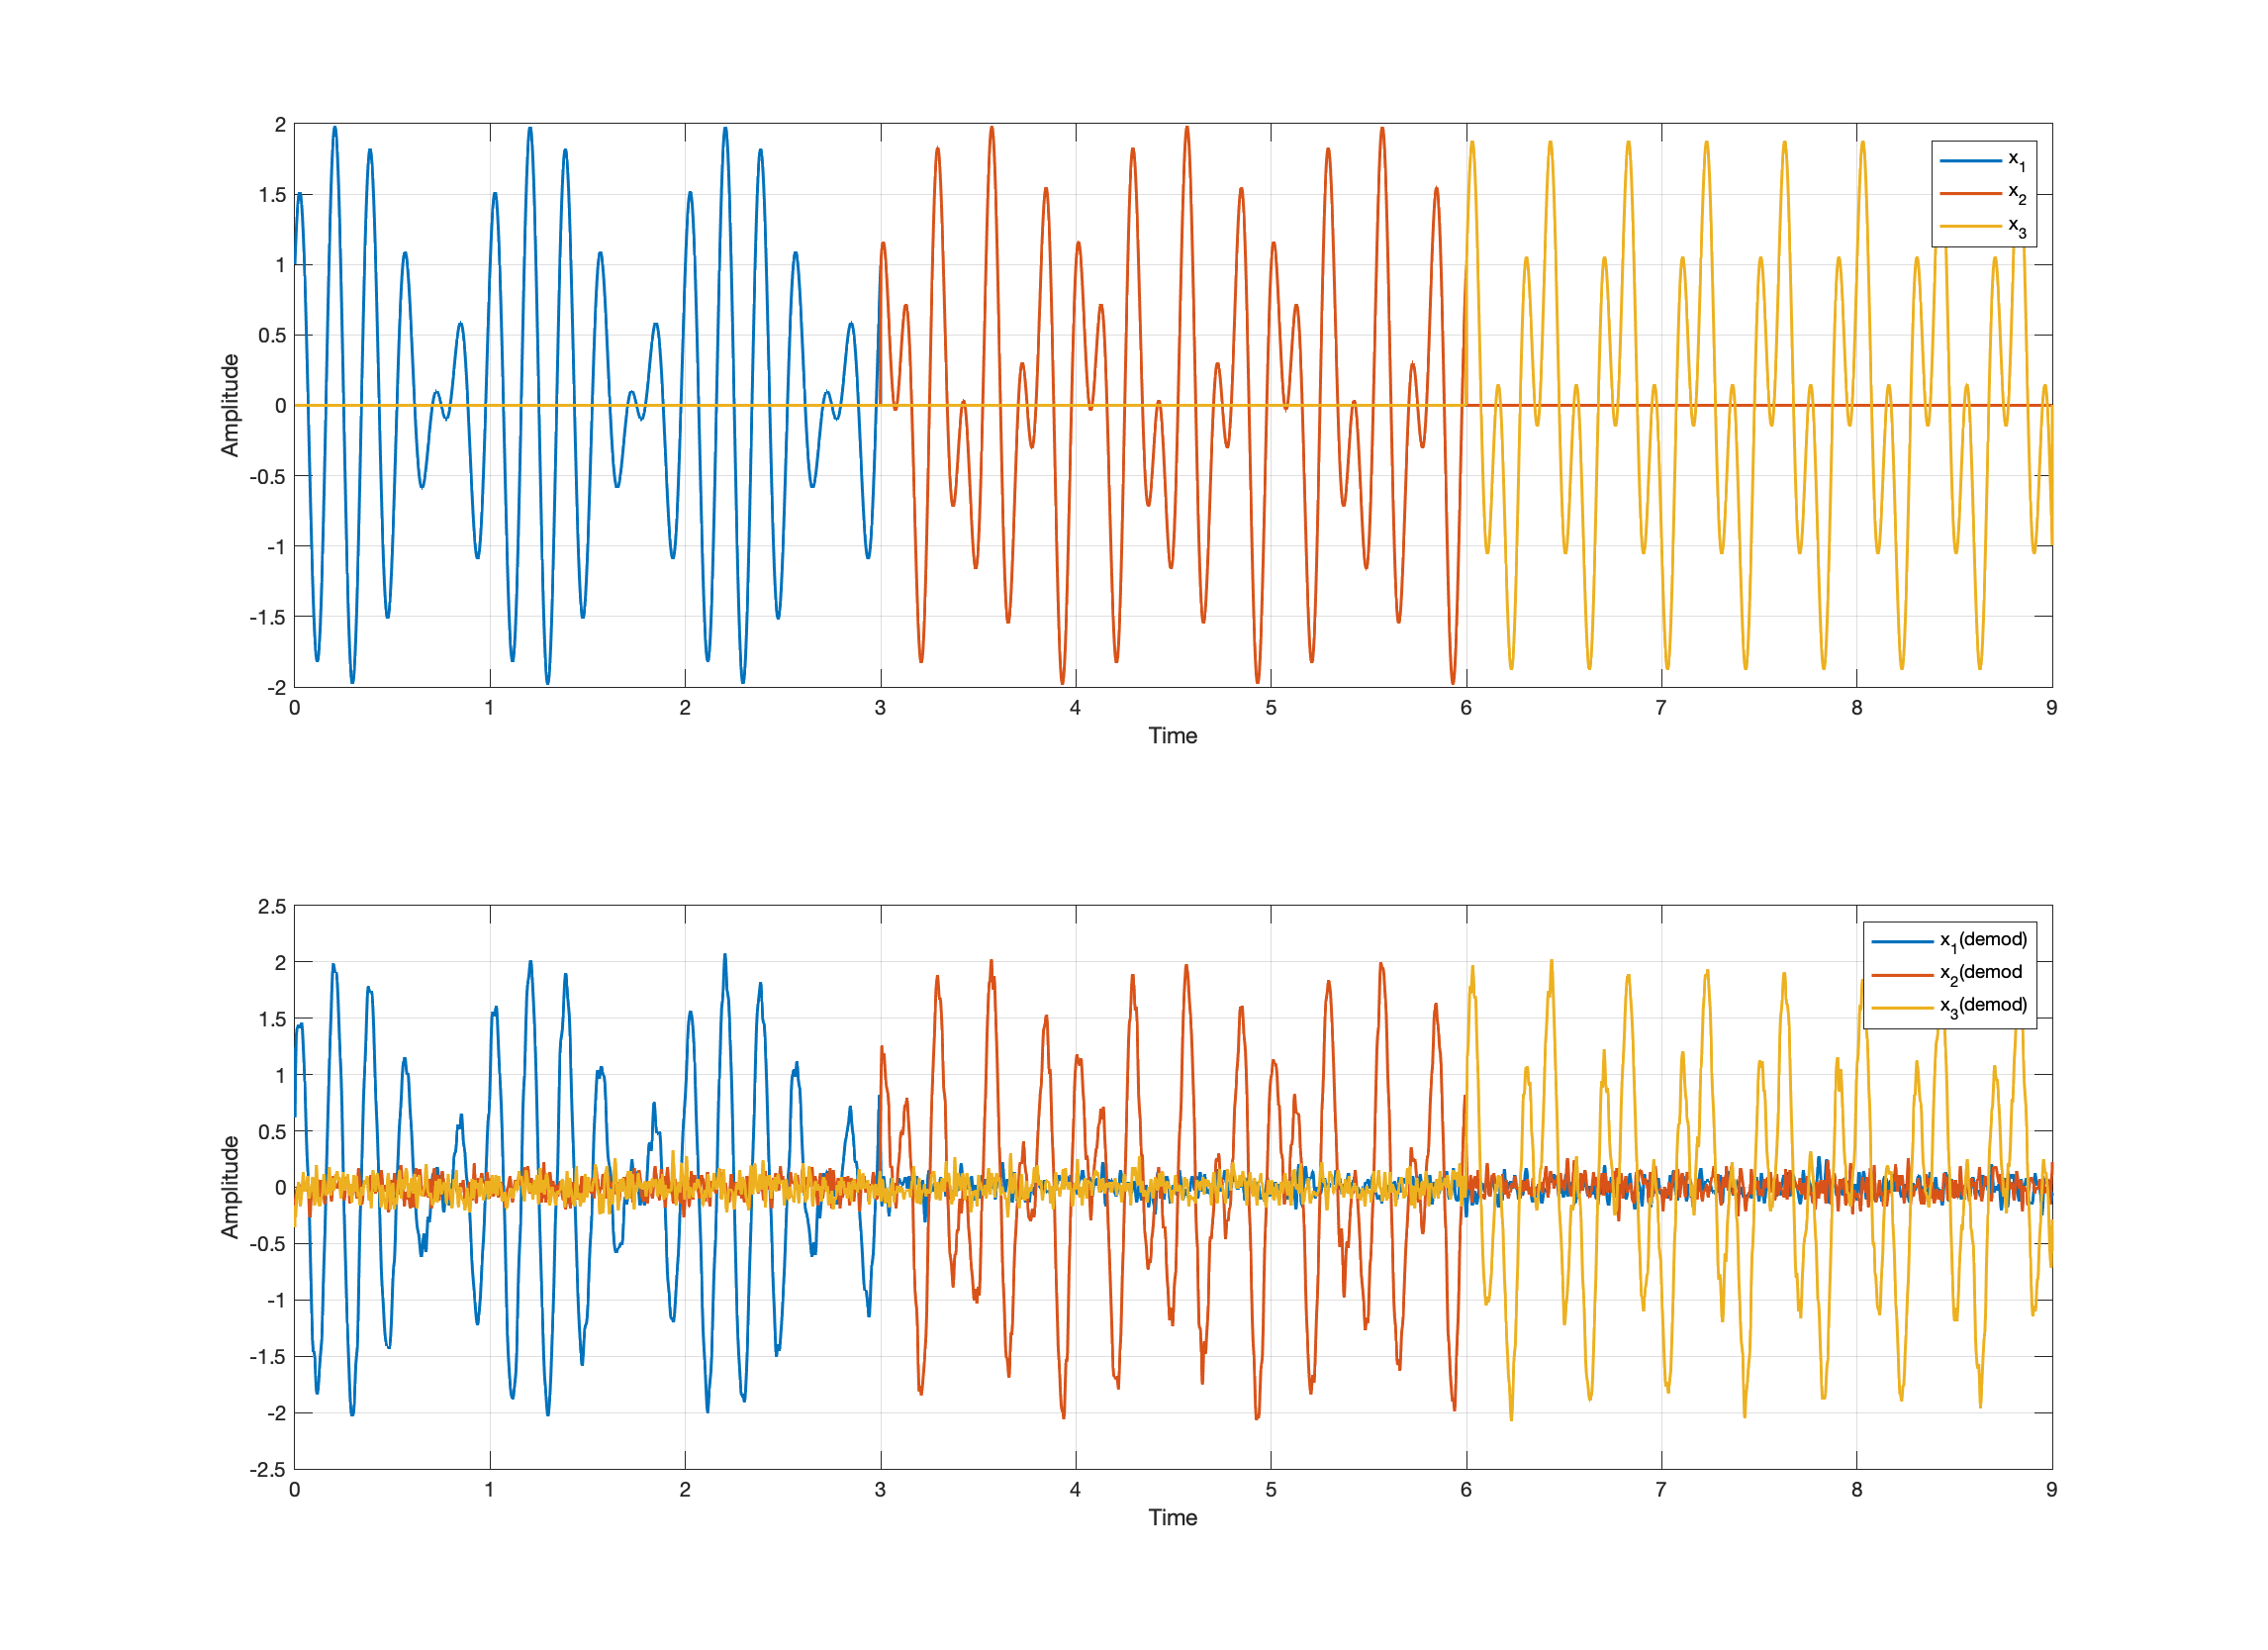
\includegraphics[width=0.62\linewidth]{../pics/q2-4-2.png}}
		\subfigure[نمودار سیگنال‌ها روی هم]{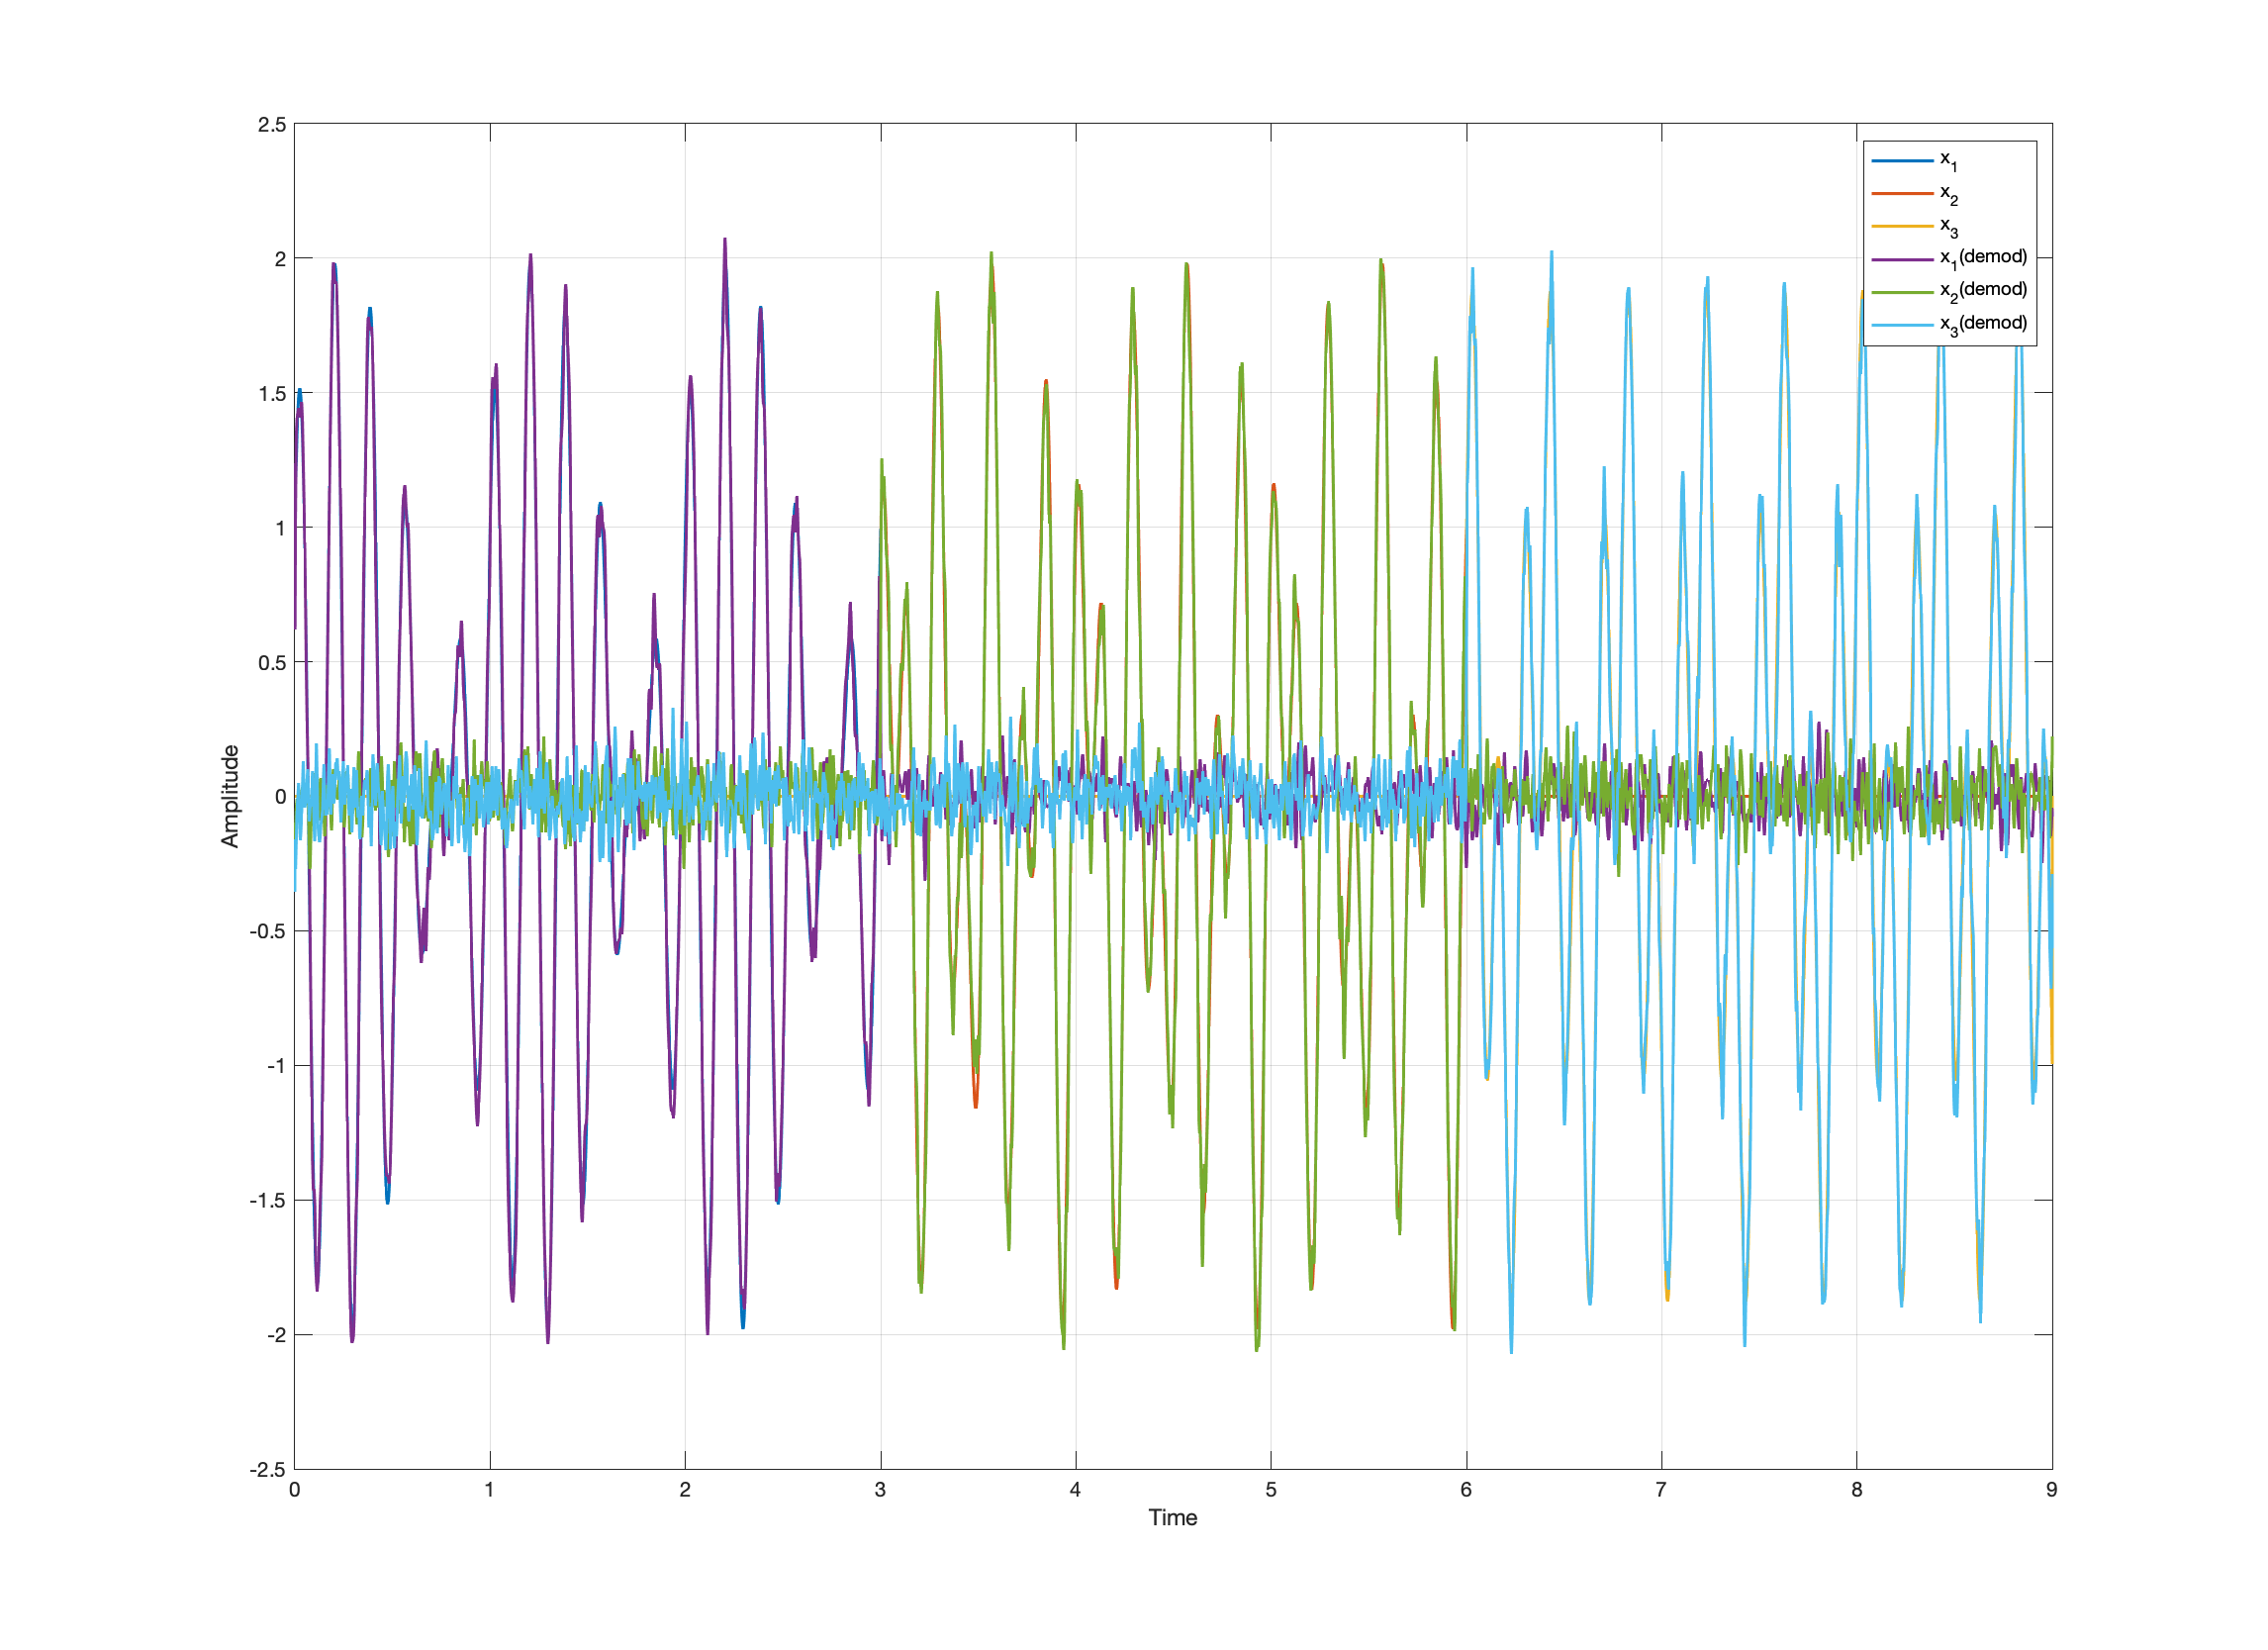
\includegraphics[width=0.62\linewidth]{../pics/q2-4-1.png}}
	\end{center}
	\caption{نمودار سیگنال‌های پیام فرستاده و دریافت شده}
\end{figure}

\noindent
همان‌طور که مشاهده می‌شود، پیام‌های استخراج شده به تقریب خوبی با پیام‌های فرستاده شده اصلی برابر می‌باشند.

\newpage
\section{\lr{FM Modulation}}
کد این سوال در فایل 
\lr{Q3.m}
قرار گرفته است. در این سوال با استفاده از سه روش، پیام مدوله شده بازیابی شده است. در روش اول از دستور 
\lr{fmdemod}
استفاده شده و به راحتی پیام مورد نظر بازیابی شده است. در روش دوم با استفاده از 
\lr{Envelope Detector}
سوال اول، پیام مورد نظر بازیابی و در نهایت در روش سوم ابتدا از یک 
\lr{Zero Crossing Detector}
استفاده شده و سپس از روی آن پالس‌های مورد نظر تولید شده است. در نهایت با استفاده از دستور 
\lr{lowpass}
یک فیلتر پایین‌گذر با فرکانس عبور ۳۰ هرتز روی این پالس اعمال شده است و با کم کردن میانگین این سیگنال از خودش و نرمالیزه کردن سیگنال نهایی، به سیگنال بازیابی شده نهایی میرسیم. در شکل زیر نمودار پیام اولیه و پیام‌های بازیابی شده با روش‌های ذکر شده در بالا قابل مشاهده است.
\begin{figure}[h]
	\centering
	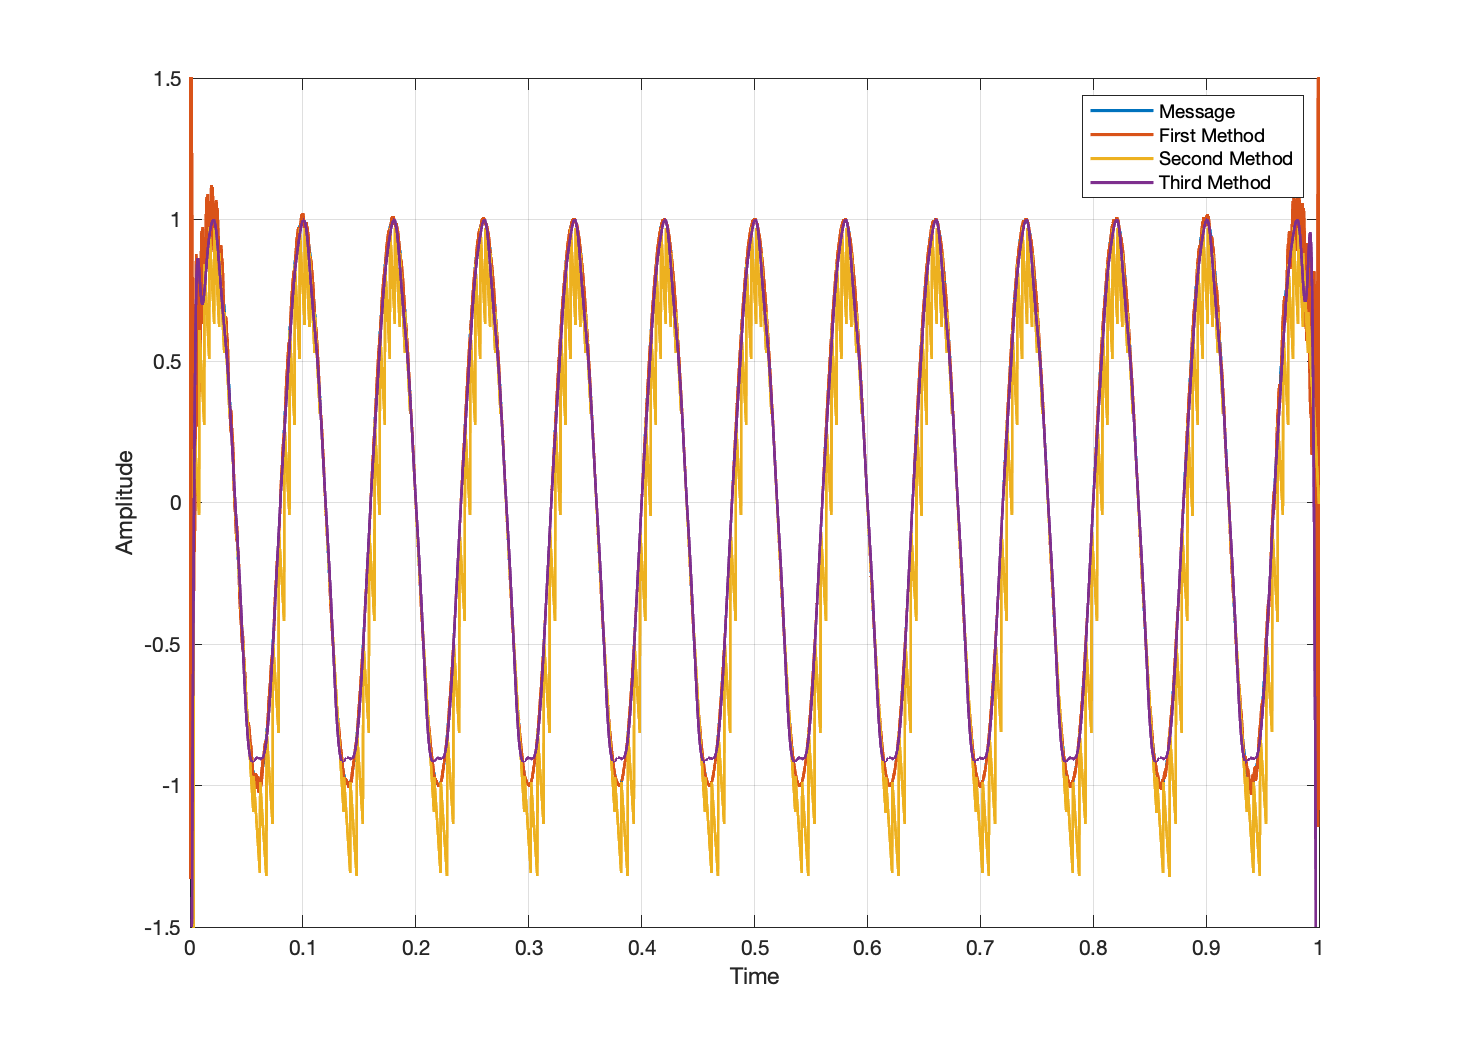
\includegraphics[width=0.9\linewidth]{../pics/q3-1}
	\caption{نمودار پیام اولیه و پیام‌های بازیابی شده}
	\label{fig:q3-1}
\end{figure}

\noindent
با توجه به نمودار بالا، روش اول یعنی استفاده از دستور 
\lr{fmdemod}
بهترین عملکرد را به نسبت بقیه روش‌ها دارد. در مقابل، روش دوم عملکرد قابل قبولی دارد اما به نسبت دو روش دیگر ضعیف تر است. همچنین روش سوم نیز عملکرد بسیار خوبی داشته و به حد خوبی سیگنال اصلی را آشکار کرده است.

\end{document}